This is an output-only problem. That means, that you don't need to submit your solution, but only need to submit outputs for given set of inputs. You can download test data in a problem materials section. It is an archive containing input files 01, 02, 03, \dots. You need to submit a single zip-archive containing your outputs 01.out, 02.out, 03.out, \dots in the root of the archive.  An archive can contain no answers for some of tests, you'll receive ``\t{Wrong Answer}'' verdict in these tests.

You are implementing an application for a mobile phone, which has a black-and-white
screen. The x-coordinates of the screen start from the left and the y-coordinates from the
top, as shown in the figures. For the application, you need various images, which are
not all of the same size. Instead of storing the images, you want to create the images
using the phone's graphics library. You may assume that at the start of drawing an
image, all pixels of the screen are white. The only graphics operation in the phone's
library is XOR(L,R,T,B), which will reverse the pixel values in the rectangle with
top left coordinate (L,T) and bottom right coordinate (R,B), where L stands for the left,
T for the top, R for the right and B for the bottom coordinate. Note that in some other
graphics libraries the order of the arguments is different.
As an example, consider the image in Figure-3. Applying XOR(2,4,2,6) to an all
white image gives the image in Figure-1. Applying XOR(3,6,4,7) to the image of
Figure-1 gives the image in Figure-2, and applying XOR(1,3,3,5) to the image in
Figure-2 finally gives the image in Figure-3.

\begin{center}
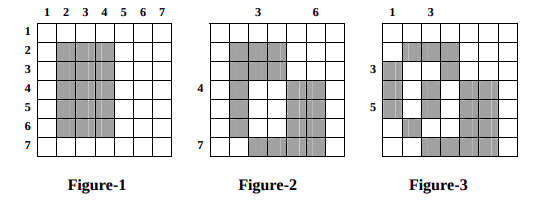
\includegraphics{1.png}
\end{center}

Given a set of black-and-white pictures, your task is to generate each picture from an
initially white screen using as few XOR calls as you can. You are given the input files
describing the images, and you are to submit files including the required XOR call
parameters, not a program to create these files.